\chapter{状態、アイデンティティ、変化}

あなたは、エンティティ、データのコレクション、ドメイン関数、およびシーケンシャルなデータを処理するためのいくつかの便利なパターンを手に入れました。そろそろ、アプリケーションの実行中におけるドメインデータの連続性について考え始める時期です。

つまり、ドメインエンティティのIDと状態、そしてドメイン内のIDがどのように関連しているかを考える必要があるのです。ドメイン内で一貫した状態管理を行うことで、第5章「コアの使用」で検討する並行処理のためのアプリケーションを準備することができます。

この章では、ドメイン内のエンティティの状態の変更を管理するためのClojureのツールの適用を学びます。より基本的には、アイデンティティと状態を別々のものとして見ていきます。Clojureは、コンピューティング世界のマルチコア状態を利用するように設計されています。状態管理の戦略を選択するための実用的なアドバイスを見つけ、マルチスレッドプログラムを考慮して、ミュータビリティがもたらす落とし穴のいくつかを認識することを学びます。

Clojureアプリケーションのコンテキストで状態とIDが何を意味するのか、その概要から始めましょう。


\section{変更のモデル化}

Clojureの焦点はimmutableな値であることを思い出してください。不変のデータでは、"更新 "は、その場のエンティティまたはエンティティを更新するのではなく、エンティティ(またはエンティティのコレクション)の新しいインスタンスを生成します。ほとんどの場合、この方法で十分に目的を果たすことができます。時には、アプリケーションの世界の変化をモデル化し、データの変化を追跡する必要があります。具体的には、変更されたデータのセットへの参照を保持する必要があります。

マルチスレッドのシナリオでは、その場でデータを更新することは、多くの複雑な問題を引き起こします。誰がデータを変更できるのか?他のスレッドにはどのように変更が通知されるのか?複数の更新が同時に発生した場合、どのプロセスが優先されるのか?Clojureは、状態管理ツールによって、これらの質問すべてにエレガントな答えを提供します。これらのツールを効果的に使用するには、まずClojureのアイデンティティと状態へのアプローチを理解する必要があります。

\subsection{スナップショットで見る}

その理解を助けるために、少し時間の話をしましょう。人間の経験は連続的に見えますが、あなたの感覚は情報を個別の量子に分けて収集しています。音、景色、匂いは、それぞれ独立して脳に入り、時間的な瞬間に相関します。その瞬間が連続して再生されることで、連続した知覚が得られると錯覚しているのです。

もし、自分の視覚的な量子を見るなら、次の図に示すエドワード・マイブリッジの「疾走するサリー・ガードナー」のようなスナップショットの連続が見えるだろう。

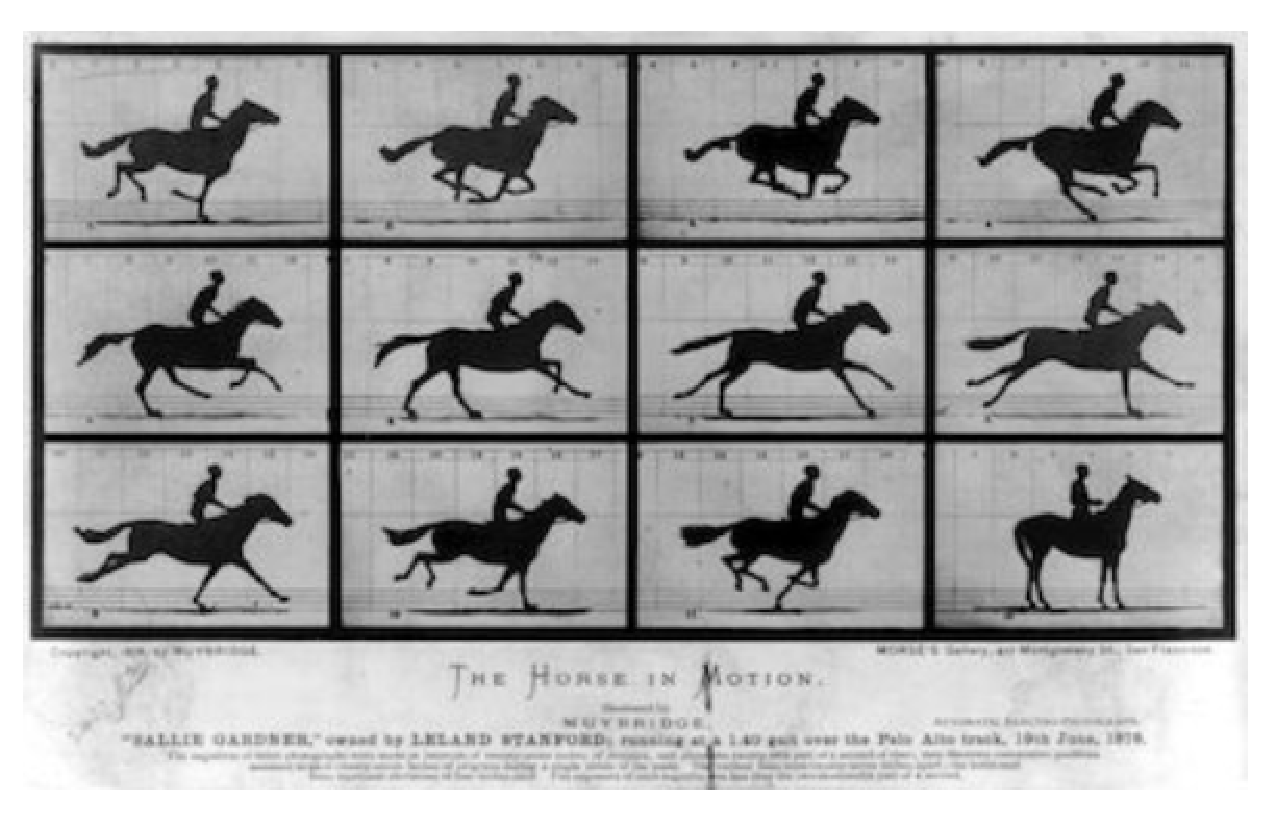
\includegraphics[width=10cm]{fig_04_001.eps}



 % Modeling a Change
\section{変更を管理するためのツール}

Clojureには、アプリケーションの状態を保存するために使用できる4つの参照型(\texttt{var}、\texttt{atom}、\texttt{agent}、\texttt{ref})があります。どの場合にも、メカニズムは、不変の値を格納するミュータブルコンテナを提供します。コンテナは初期値で作成し、その値をリセットすることができます。また、統一更新モデルを用いて状態を進めることもできる。このようにして、アプリケーションの状態を管理された方法で変更することができる。

Clojureの参照型は\texttt{IRef}を実装しています。次の表は、これらの型と、それらの作成、更新、およびリセット関数の一覧です。

\begin{tabular}{|l|l|l|l|}
\hline
IRef & create-fn & update-fn(s) & set-fn \\ \hline \hline
Atom & atom & swap! & reset! \\ \hline
Ref & ref & alter, commute & ref-set \\ \hline
Var & def & alter-var-root & var-set \\ \hline
Agent & agent & send, send-off & restart-agent \\ \hline
\end{tabular}

これらのリファレンスタイプはどれも似たようなパターンです。


\begin{lstlisting}[numbers=none]
;; 作成
(create-fn container)
;; 更新
(update-fn container data-fn & args)
;; 値を設定する
(set-fn container new-val)
\end{lstlisting}

エージェントの場合、作成時にエラー処理オプションを含めることができます。

\texttt{var} はローカルメモリに変更可能なデータを保存し、管理されません。\texttt{atom}は、同期変換(\texttt{swap!}を使用)により保存された値の変更を制限しますが、これらの変更を調整することはありません。\texttt{Ref}は、STMによって、保存された値の制御された変換を提供します。\texttt{agent}は個々のアプリケーションの状態を保存するが、非同期で更新する。(このセクションでは、\texttt{atom}、\texttt{ref}、および \texttt{var} の概要と、それらの使用方法を示す例について説明します。

まず、\texttt{atom}や\texttt{ref}を使用した変更の管理に注目しましょう。


\subsection{Atomによるマネージドアップデート}

データが複数のスレッドによって観測され始めると、それらのスレッドを、調整されていない部分的な更新の混乱から守ることが必要になります。これを怠ると、システムが無効な状態に陥る可能性がある。



\subsubsection{買い物に行こう}

アクティビティをどのようにコーディネートするのがベストなのか、思考を巡らせてみましょう。同時進行の実装を決定するたびに、どの情報を管理し、どの情報を管理しないようにするかを決めるために、同様の演習を行うことになります。

練習のために、食料品の買い物に出かけましょう。まず、シングルスレッドで買い物をすることを考え、次にそのニーズを基に、より複雑なマルチスレッドの例を考えてみましょう。続けて、有用なものができるまで、様々なトランザクションメモリメカニズムを追加していきます。

\subsubsection{ソロオペレーター}

私たちは、食料品の買い物がどのように行われるかを知っています。リストを作り、店に行き、リストにあるものを買うのです。一人の場合、これはとても簡単なことです。リストを作った人が買い物に向かいます。


\begin{lstlisting}[numbers=none]
(defn go-shopping-naive
  "購入した商品の一覧を返します。"
  [shopping-list]
  (loop [[item & items] shopping-list
         cart []]
    (if item
       (recur items (conj cart item))
       cart)))
\end{lstlisting}


このシナリオでは、状態管理は必要ない。1つのスレッド(人)がリストをたどり、おいしいジャンクフードでいっぱいのカートを返します。少なくとも、あなたが大学生の時はそうでしたね。

この例では、すべてが無限の棚に置かれています。私たちは単に、あるリストから別のリストへ物を移動しているだけです。もっと完全な表現にすると、店の在庫を表すことになり、大学生は寮の友達が先にすべてのピザを手に入れたことを発見するかもしれません。その在庫を管理できるようなAPIを書いてみよう。

\subsubsection{ストアAPIの構築}

私たちの店の在庫を、商品と数量のマップとして表現する。複数のスレッドがこの在庫を操作することが予想されるので、どのオブザーバーも一貫したデータを見ることができるようにする必要があります。これは\texttt{atom}で実装することができます。

\texttt{atom}は同期された構造体です。つまり、\texttt{atom}を使用することで、\texttt{atom}に加えたすべての変更が、次の変更が適用される前に完全に行われることを保証します。また、\texttt{atom}は独立であり、非協調でもあります。調整については、次のセクションでもう少し詳しく説明します。最後に、\texttt{atom}はすぐに更新されます。ストアに加え、\texttt{grab}関数と\texttt{stock}関数を定義して、我々の新生APIを形づくることにしよう。


\begin{lstlisting}[numbers=none]
(ns shopping.store)

(def inventory (atom {}))

(defn no-negative-values?
  "マップの値が負であるかどうかをチェックする"
  [m]
  (not-any? neg? (vals m)))

(defn in-stock?
  "在庫を確認する"
  [item]
  (let [cnt (item @inventory)]
    (and (pos? cnt))))

(defn init
"在庫を持つ店舗を構える。"
[items]
(set-validator! inventory no-negative-values?)
(swap! inventory items))

(defn grab
  "棚から品物を取ってくる。"
  [item]
  (if (in-stock? item)
    (swap! inventory update-in [item] dec)))

(defn stock
  "棚に商品を仕入れる"
  [item]
  (swap! inventory update-in [item] inc))
\end{lstlisting}

\texttt{atom}関数を用いて、インベントリがアトムであることを宣言し、その値の変更は、その変更を管理できる関数に限定されることを宣言している。これらの関数は \texttt{swap!}、\texttt{reset!}、さらに低いレベルでは \texttt{compare-and-set!}

インベントリの値はアトム内に格納されているので、値を見るには \texttt{(deref inventory)} または \texttt{@inventory} で参照する必要があります。アトムの値を変更するとき、Clojureは隠れて次のようなことをします。


\begin{enumerate}
\item 現在値をデリファレンス(保存)する
\item \texttt{swap!}に渡された関数を呼び出す.
\item 新しい値を検証するか、例外をスローする
\end{enumerate}

\begin{enumerate}
\item 比較検討する。

\begin{itemize}
\item 参照の現在値が(例えば他のスレッドによって)変更されていない場合、関数の呼び出し結果で置き換え、新しい値を返す。

\item 現在の値がメソッド呼び出し中に変更された場合は、値を置き換えず、最初からやり直します。
\end{itemize}
\end{enumerate}


\subsubsection{無効な状態に対する保護}

\texttt{swap!}メソッドは任務が完了するまで繰り返されます。データの完全なスナップショットに対して関数を呼び出すことが保証されています。しかし、\texttt{swap!}が呼び出されたときにアトムが持っていた値に対して関数を呼び出すことは保証されていない。16行目で定義したバリデータがなければ、負の\texttt{:bacon}が生成される可能性がありますし、誰もそれを望んでいません。このような不運なタイミングの例を見てみましょう。


\begin{lstlisting}[numbers=none]
(:bacon @inventory)                          ;=>1
(if (in-stock? item)                         ; thread 1
(if (in-stock? item)                         ; thread 2
    (swap! inventory update-in [item] dec))) ; thread 2
    (swap! inventory update-in [item] dec))) ; thread 1
(:bacon @inventory)                          ;=>-1
\end{lstlisting}

このように、ガードのタイミングが重要なのです。在庫がマイナスにならないようにするために、19行目でバリデータ関数を渡して保険をかける必要があります。バリデータを使うことで、在庫アイテムの持つ最小値が0であることを保証できます。

アトムの値が変更される前に、新しい値の候補がバリデータ関数に渡されます。バリデータ関数が \texttt{false} を返した場合、アトムを変更しようとすると \texttt{IllegalStateException} がスローされます。バリデータ関数は独自の例外をスローすることも可能で、 その場合は \texttt{IllegalStateException} の代わりとなります。これが可能な場合 (たとえば、\texttt{store.clj} の 22 行目から \texttt{grab} 関数を呼び出す場合)、その可能性に対処する必要があります。一般に、バリデータは単一の引数を取る副作用のない関数 (または \texttt{nil}) でなければなりません。この関数は何度も呼び出すことができることを思い出してください。

(インベントリを定義するときにバリデータ関数を宣言することも簡単にできます。


\begin{lstlisting}[numbers=none]
(def inventory (atom {} :validator no-negative-values?))
\end{lstlisting}

これは、特に初期状態を渡す場合に便利です。バリデータはアトム生成時に初期状態を検証します)。

さて、エマージェント・ストアAPIを使い、ループを\texttt{reduce}に置き換えることで、よりすっきりしたアプローチになりました。このコードは\texttt{go-shopping-naive}関数を置き換えます。


\begin{lstlisting}[numbers=none]
(defn shop-for-item [cart item]
  "商品を購入し、カートを更新して戻る。"
  (if (store/grab item)
    (conj cart item)
    cart))

(defn go-shopping
  "購入した商品の一覧を返します。"
  [shopping-list]
  (reduce shop-for-item [] shopping-list))
\end{lstlisting}

このシンプルな例でも、いくつかの熟考されたステップを経て、APIが形作られ始めていることに注目してください。このようなことは、いつでもどこでも起こっているはずです。考えて、実行して、小さな驚きが生まれるのです。


\subsection{在庫を見る}

毎週毎週、大学生にラーメンを食べさせるためには、お店は定期的に補充をしなければなりません。マスターリストや設定ファイルから定期的に補充することも可能ですが、その場合、スケジュールを気にする必要があります。そこで、「見る(ウォッチ)」機能を追加することを検討してみてはどうだろう。

ウォッチは、物事を監視するために存在します。これは、オブジェクト指向言語におけるObserverデザインパターンの実装に相当するもので、ほとんど同じ目的を果たす。しかし、ウォッチにはほとんどオーバーヘッドがありません。Clojureはウォッチの登録と通知を処理するので、ウォッチャー関数は単純な関数のままです-具体的には、キー、ウォッチへの参照、古い値、新しい値という4つの引数からなる関数です。

ウォッチ機能は、すべての参照型に適用できる。一つの参照に複数のウォッチャーを持つことができ、それぞれが異なるキーを持ち、参照される値が変更されると、すべてのウォッチャーが更新されます。

例を挙げましょう。例えば、ある商品が在庫からなくなったときに、店に通知するためにウォッチ関数を使用するとします。


\begin{lstlisting}[]
(declare sold-items)

(defn restock-order
  "再入荷ウォッチ"
  [k r ov nv]
  (doseq [item (for [kw (keys ov)
                     :when (not= (kw ov) (kw nv))] kw)]
    (swap! sold-items update-in [item] (fnil inc 0))
    (println "need to restock" item)))

(defn init-with-restock
  "店舗を構え、在庫を持つ"
  [m]
  (def inventory (atom m))
  (def sold-items (atom {}))
  (set-validator! inventory no-negative-values?)
  (add-watch inventory :restock restock-order))
\end{lstlisting}

イニシャライザーを変更し、17行目にウォッチ関数を追加しています。ウォッチ関数は次のような形式をとります。

\begin{lstlisting}[numbers=none]
(defn watch-fn [watch-key reference old-value new-value] ,,,)
\end{lstlisting}

このメソッドは、アトムの値が正常に更新されるたびに呼び出されます。古いインベントリ値と新しいインベントリ値を比較し、変更されたアイテムを新しいアトムである\texttt{sold-items}に抽出します。\texttt{grab}は一度に1つのアイテムしか取り出さないことが分かっているので、単純なインクリメントで満足できます。

ウォッチ関数は4つのパラメータを取ります。関数のキー、ウォッチされる参照、古い値、新しい値です。最後の3つは簡単ですが、キー(例えば\texttt{:restock})は不透明な場合があります。裏を返せば、このキーはリファレンスに付けられたウォッチ関数のハッシュマップの中でウォッチ関数を特定するものです(\texttt{.getWatches}関数で取得可能)。このキーは \texttt{remove-watch} でウォッチ関数を削除したり、\texttt{add-watch} で既存のウォッチ関数を置き換えたりするのに使用されます。一般に、キーはラベルとして扱うことができ、あまり気にする必要はありません。

これで、棚から商品が取り出されたことを検出できるようになったので、棚を補充してみましょう。

\subsection{棚の再入荷}

売れた商品を記録するようになったら、定期的に棚を補充したくなるかもしれません。ここでは、かなり地味な補充方法を実装することにする。在庫と売れた商品の両方をリセットします。



\begin{lstlisting}[numbers=none]
(defn restock-all
  "restock all items sold" 3 []
  (swap! inventory #(merge-with + % @sold-items))
  (reset! sold-items {}))
  ; be careful, here be dragons.
\end{lstlisting}

でも、ちょっと待ってください! このようにシンプルにしすぎたために、いくつかの重要なことを見逃しています。ストアのAPIを使うと、それがすぐにわかります。


\begin{lstlisting}[numbers=none]
user=> (use ['shopping.store :as 'store])
nil
user=> (store/init-with-restock {:apples 1 :bacon 3 :milk 2})
#<Atom@eb74118: {:bacon 3, :apples 1, :milk 2}>
user=> (store/grab :bacon)
need to restock :bacon
user=> (store/grab :bacon)
need to restock :bacon
{:bacon 1, :apples 1, :milk 2}
user=> (store/grab :milk)
need to restock :milk
{:bacon 1, :apples 1, :milk 1}
user=> @store/sold-items
{:milk 1, :bacon 2}
user=> @store/inventory
{:bacon 1, :apples 1, :milk 1}
user=> (store/restock-all)
need to restock :bacon
need to restock :milk
\end{lstlisting}

先ほどのセッションで出力された最後の2行は、私たちの見落としの一つを示すものです。\texttt{restock-all}の中で\texttt{swap!}を使って在庫を更新したとき、ウォッチ関数が呼び出され、売れた商品のリストに新しい項目が2つできました。なぜ、3つではなく2つなのでしょうか?なぜなら、ウォッチ関数は数量の変化を調べるようには設計されておらず、売れた商品の名前だけを記録するように設計されていたからです。同じことが、stockを呼び出した場合にも起こります。

もうひとつの見落としは、もう少し曖昧なままです。私たちは、この世界を同時並行的に理解しようとしていることを思い出してください。\texttt{restock-all}関数では、5行目の直前にカオスが入り込む隙間ができています。もし他のスレッドがその時にインベントリからアイテムを取ってきたら、\texttt{sold-items}アトム内のそのアイテムのエントリは消去され、次に再入荷する時にアイテムが不足することになります。

この場合、インベントリ・コンテナのアトム選びは失敗したことになる。この実装では、在庫は独立して同期的に追跡されることを意図していた。しかし、2つ目のアイテム追跡機構を追加すると、突然、物事を調整する必要が生じます。たとえ少数のものでも調整するのは難しい。このトリッキーさには \texttt{refs} を使って対処できます。

\subsection{Refによるトランザクションの変更}

より複雑なドメインでは、複数の値の同時更新を調整する必要があるため、アトムはもはや機能しません。トランザクションの力が必要であり、それには一連の参照関数が必要である。これを複雑な買い物の例で示そう。


\subsubsection{パックでお買い物}


お子さんがいらっしゃる方は、お子さんを連れてきてカートに入れるのを手伝ってもらうといいかもしれませんね。この場合、ある程度の連携が必要になるので、どのようなやり方が最適かを決める必要があります。

簡単なシナリオとしては、買い物リストを子どもたちに分担させ、各自のリストにある商品を取りに行かせます。買い物を終えた子どもたちが戻ってきたら、最後に商品を組み合わせます。

これで問題解決ですね。役割分担をすることで、コーディネートの問題を先に解決し、その後の協力は不要になったのです。状態管理:回避

もちろん、これは子供たち全員が同じ注意力を持っていて、リストにあるものを見つけるためにベストを尽くし、気が散らないようにし、他のものを持ち帰らないことを前提としています。もしこれがすべて真実であれば、物事は順調に進むと期待できます。子供の買い物へのアプローチをより現実的に実行すると、次のようになります。



\begin{lstlisting}[numbers=none]
(defn dawdle
  "ぶらぶらしたり、迷子になったり、お菓子を買ったり"
  []
  (let [t (rand-int 5000)]
    (Thread/sleep t)
    (maybe? buy-candy)
    ))
\end{lstlisting}

ちょっとしたカオスが加わったので、それを緩和する必要があります。子どもたちを1つずつ探しに行かせ、ある程度の時間、ぐずぐずさせます。戻ってきたら、その商品とお菓子をカートに入れ、次の課題を受け取ります。集中力のある子供たちは、より多くの仕事をこなしますが、アイテムは最終的にリストから取り除かれます。

\subsubsection{ルールからトランザクションを構築する}

ここでの成功の鍵は、買い物をする商品に関する明確なルールを持つことです。そのルールがあれば、そのルールに従ったモデル化と状態の更新を行いたい。

ルールは簡単だ。

\begin{itemize}
\item 買い物リストのアイテムは、子供に割り当てられると消去される。

\item カートに入れるまで、その商品は子供に割り当てられたままです。

\item お菓子は買い物リストにもカートにも入れられません。
\end{itemize}

我々のルールを守るために、ローカルな世界から見て、子供に品物を割り当てることと、買い物リストから取り除くことは同時に行われなければなりません。同様に、商品を回収することと、カートに入れることも、事実上同時に行わなければならない。これらの動作を調整するために、1つまたは3つの参照が必要です。

\texttt{ref} はその値を \texttt{ref world} に保存し、その値への変更がトランザクションとして協調的かつ同期的に実行されることを保証するのに役立ちます。次の例では、3つの\texttt{ref}を作成しています。\texttt{shopping-list}は買い物をする予定のアイテムを保持するセットである.子供の名前をマップキーとして、割り当てマップで飛行中のアイテムを追跡する。最後に、ショッピングカートは、子供から回収したアイテムのセットである。


\begin{lstlisting}[numbers=none]
(def shopping-list (ref #{}))
(def assignments (ref {}))
(def shopping-cart (ref #{}))

(defn init []
  (store/init {:eggs 2 :bacon 3 :apples 3
               :candy 5 :soda 2 :milk 1
               :bread 3 :carrots 1 :potatoes 1
               :cheese 3})
  (dosync
    (ref-set shopping-list #{:milk :butter :bacon :eggs
                             :carrots :potatoes :cheese :apples})
    (ref-set assignments {})
    (ref-set shopping-cart #{})))
\end{lstlisting}

\texttt{ref}の値の変更は、\texttt{dosync}を使用して、トランザクションの内部で行わなければなりません。トランザクションは多くの更新で構成されます。

これらの更新には3つの種類があります。\texttt{ref}の値を直接更新する場合、\texttt{ref-set}を使用します。関数を使用して更新する場合は、\texttt{alter} または \texttt{commute} を使用します。最も頻繁に見るのは、再初期化のコンテキストで \texttt{ref-set} を見ることでしょう。

\texttt{alter}を使用する場合、関数を適用したときの\texttt{ref}の値が、トランザクションの開始時、または現在のトランザクション内で最後に\texttt{alter}関数が適用されたときの\texttt{ref}の値と同じであることが必要です。このトランザクションの実行中に、同時に実行されているトランザクションによって \texttt{ref} が更新された場合、再試行のトリガとなります。トランザクションが外部からの干渉を受けずに実行される必要がある場合、\texttt{alter} 関数は使用すべき関数です。

トランザクションが内部一貫性のチェックを必要としない場合、\texttt{commute}を使用することができます。\texttt{commute}関数は、トランザクションの実行中に\texttt{ref}の値が変更されても、再試行の引き金にはなりません。\texttt{commute}に渡された関数は、\texttt{ref}がその時点で持っているどのような値に対しても実行されます。

同時実行性の高いアプリケーションでは、可能な限り \texttt{alter} 呼び出しを \texttt{commute} に置き換えることで、再試行を回避して性能を向上させることができます。これは、\texttt{commute} に渡される関数が可換である場合、つまり、更新関数を適用した結果が実行順序に関係なく同じ結果になる場合にのみ実行されるべきです。足し算を考えてみてください。(4 + 6 + 2)は(2 + 4 + 6)と同じになります。

\texttt{ensure}関数は、\texttt{ref}の値が更新されずに現在のトランザクションの外で変更されていないことを確認するために使用することができます。値が変更されたことを確認した場合、再試行を開始します。これは、\texttt{ref} が相互に依存した値を持つような状況で有用です。例えば、購入を完了するとき、価格を更新していないにもかかわらず、トランザクション中に価格が変更されていないことを確認するために、価格リスト上で\texttt{secure}を行うかもしれません。トランザクションの途中で価格が変更された場合、再試行が行われるはずです。

\texttt{ref} の更新の構文を簡単に説明すると、更新を行う関数と引数を送信することで \texttt{ref} を変更(またはコミット)します。

次のコードブロックでは、トランザクションを実行するために必要な関数を定義しています。もう一度言いますが、このコードからAPIが生まれ始めているのがわかります。\texttt{assign-item-to-child} 関数は、ショッピングリストからアイテムを削除し、それを子に割り当てます。\texttt{collect-assignment}関数は、ショッピング・カートに買い物した商品を追加し、子プロセスの割り当てを破棄します。先ほどの\texttt{dawdle}関数は\texttt{buy-candy}を使用しています。以下はトランザクションです。


\begin{lstlisting}[numbers=none]
(defn assignment
  [child]
  (get @assignments child))

(defn buy-candy []
  (dosync
    (commute shopping-cart conj (store/grab :candy))))

(defn collect-assignment
  [child]
  (let [item (assignment child)]
    (dosync
      (alter shopping-cart conj item)
      (alter assignments dissoc child)
      (ensure shopping-list) ;; not needed
                             ;; included as an example
      )
    item))

(defn assign-item-to-child [child]
  (let [item (first @shopping-list)]
    (dosync
      (alter assignments assoc child item)
      (alter shopping-list disj item))
    item))
\end{lstlisting}

前述のメソッドはいずれも、ローカル制御が戻る前に完全に更新する必要がある、状態の2つの異なる要素に対して操作します。これらのメソッドは、\texttt{alter} を使用して、変更されるコレクションを更新し、操作がこの順序で実行されることを示します。また、更新されなかった参照を保護するために \texttt{ensure} を使用します。

トランザクション(\texttt{dosync})が実行されている間、\texttt{dosync}ブロックで特定された参照への書き込みは防止されます。これらの変更はすべて提案され、次に代替タイムラインである \texttt{ref} の世界にコミットされます。すべてが正常に終了した場合、すべての更新は書き込みポイントの後にローカルワールドで読むことができるようになります。そうでなければ、変更はコミットされず、トランザクションは再試行回数制限(この記事の執筆時点では10,000回)に達するまで再試行されます。これにより、実行中のすべてのスレッドで我々のルールが維持されることが保証されます。


\subsubsection{買い物に行く}

さて、トランザクションメソッドの定義ができたので、実際に買い物に行くことができます。


\begin{lstlisting}[numbers=none]
(defn send-child-for-item
  "eventually shop for an item"
  [child item q]
  (println child "is searching for" item)
  (dawdle)
  (collect-assignment child)
  (>!! q child))

(defn report []
  (println "store inventory" @store/inventory)
  (println "shopping-list" @shopping-list)
  (println "assignments" @assignments)
  (println "shopping-cart" @shopping-cart))

(defn go-shopping []
  (init)
  (report)
  (let [kids (chan 10)]
    (doseq [k my-kids]
      (>!! kids k))
    (go-loop [kid (<! kids)]
      (if (seq @shopping-list)
      (do
        (go
          (send-child-for-item kid (assign-item-to-child kid) kids))
        (recur (<! kids)))
      (do
        (println "done shopping.")
        (report))))))
\end{lstlisting}

\texttt{go-loop}や奇妙なエイリアンのアルファベット(\texttt{<!}, \texttt{>!})に見覚えがあっても心配しないでください。これらは\texttt{core.async}の一部で、第5章「コアの使用」で並行処理について説明するときに詳しく説明します。今のところ、ループを開始するときにキューから子オブジェクトを取得し(チャネルと呼ばれます)、その子オブジェクトに割り当てられたアイテムを収集した後にキューに戻すということを知っておいてください。

それ以外は、買い物そのものはかなり直感的に進められる。トランザクションをできるだけシンプルに、できるだけ少ない場所で行うことで、カオスになるリスクの多くを軽減しています。

そういえば、お菓子の話はしていませんでしたね。ルールではお菓子はダメなので、バリデーターをショッピングカートに追加しましょう。


\begin{lstlisting}[numbers=none]
(def shopping-cart (ref #{}
  :validator #(not (contains? % :candy))))
\end{lstlisting}

また、どうしてもお菓子が入ってしまったときにカートを爆発させたくなければ、それが起きたときに親に通知する監視機能を追加して、罰に関する判断を遅らせることもできます。


\begin{lstlisting}[numbers=none]
(defn notify-parent
  [k r _ nv]
  (if (contains? nv :candy)
    (println "there's candy in the cart!")))
\end{lstlisting}

ウォッチ機能を作成したら、initでショッピングカートに追加します。


\begin{lstlisting}[numbers=none]
(add-watch shopping-cart :candy notify-parent)
\end{lstlisting}

最後に、varコンテナについて考えてみましょう。





\subsubsection{Varでローカルな状態を追跡する}

最後に、すべての状態について管理が必要なわけではありません。変更されないデータ(システムの状態など)には変更管理は必要ありません。同様に、他のスレッドから観測されないデータも管理する必要はありません。このような場合、データを保存するためにvarを使用します。\texttt{def}を使って、var を設定する:


\begin{lstlisting}[numbers=none]
user=> (def my-kids #{:alice :bobby :cindi})
\end{lstlisting}

このvarは、現在の名前空間内のシンボル(\texttt{my-kids})を持つグローバルなスコープを持つ。もしその var がすでに存在すれば、新しい値が設定される。この var は好きなように読み込んで再定義することができます。\texttt{alter-var-root} を使って、var を更新します。\texttt{my-kids} の前の \texttt{\#'} に注意してください: \texttt{alter-var-root} には、その値ではなく、var 自体を渡します。


\begin{lstlisting}[numbers=none]
user=> (defn born! [new-kid] (alter-var-root #'my-kids conj new-kid))
#'user/born!
user=> (born! :donnie)
#{:donnie :alice :bobby :cindi}
\end{lstlisting}

グローバルな定義を損なうことなく、ローカルバインディングやスレッドでvarを再定義できるようにしたい場合、定義時にこの効果を持たせるためのメタデータを追加することが可能です。


\begin{lstlisting}[numbers=none]
user=> (def ^:dynamic my-kids #{:alice :bobby :cindi})
#'user/my-kids
user=> (print my-kids)
#{:alice :bobby :cindi}
user=> (binding [my-kids #{:luke :leia}]
#_=>     (print my-kids))
#{:leia :luke}
user=> (print my-kids)
#{:alice :bobby :cindi}
\end{lstlisting}

Varsはステートフルですが、ローカルメモリに保存されるため、管理されることはありません。var に動的スコープを追加すると、そのバインディングはローカライズされますが、別の問題が発生します。Stuart Sierra はこの問題について "On the Perils of Dynamic Scope" という記事を書いています[18] 要するに、本当にそう思っていて、自分が何をしているのか分かっていない限り、この方法はとらない方がいいということです。

我々は、Clojureがrefとatomとそれらに関連する更新関数でアプリケーションの状態の変更を管理するために提供する主要な構造のほとんどを歩いてきました。また、グローバルな状態を保存するための var も簡単にレビューしました。さて、変更を管理するためのツールを手に入れたので、どのように変更と付き合っていくかについて少し話をしましょう。

次のセクションでは、管理された変更に関する適切な実装上の決定を行う方法と、変更可能性の影響を制限しながらAPIを成長させるための2つのアプローチについて学びます。 % Tools for Managing Change
\section{変化と生きる}

Clojureが提供する、アプリケーションの状態を更新するためのツールをいくつか詳しく見てきました。これらのツールは、変更が有効であり、瞬時に見えることを保証することで、不運から守ってくれます。しかし、まだずさんな考えで自分自身の足を撃つことができます。

状態管理の複雑さを、ドキュメントやブログ記事、そしてこの本のようなおもちゃのようなコードで示すことは困難です。しかし、これまで見てきたような仕組みを応用する際には、いくつかのガイドラインを心に留めておくとよいでしょう。

\subsection{バリデーションの方法とタイミング}

私たちの\texttt{shopping.store} APIは、冗長性と少し厄介な部分を含んでいます。\texttt{init}では、私たちのAPI(特に\texttt{grab})を無視してストアの\texttt{inventory}を直接更新するコードから保護するために、バリデータ関数として在庫に\texttt{no-negative-values?}関数を適用しました。

このバリデータメソッドは、マップのすべての要素を検査して、在庫が増加していることを確認します。在庫が大きくなり始めたらどうなるのでしょうか?\texttt{grab}で使っている\texttt{in-stock?}テストと比較して、どれだけのオーバーヘッドになるでしょうか?厄介なことに加えて、冗長です。\texttt{grab}を使おうが使うまいが、バリデータは呼び出されるのです。

どうすればいいでしょうか?少なくとも、\texttt{inventory}の\texttt{def}に \texttt{\^\{:private true\}} を追加して、\texttt{grab} の使用を奨励すべきです。より堅牢な解決策は、システムを初期化する関数を構築し、それを必要とするコンポーネントに渡すことです。これは、第7章「アプリケーションを構成する」で詳しく説明するコンポジションの水域に足を踏み入れることになります。

APIを開発する際には、必要と思われるすべてのアクションをラップした一連の関数を提供し、実際のデータの保存は非公開にするようにしましょう。こうすることで、提供された関数をバイパスして直接データを操作することを防ぐことができます。これにより、バリデータのパフォーマンスが低下するような場面でも、 不正な操作から保護する仕組みを導入することができます。バリデータ関数は Clojure がトランザクションをコミットする前に実行されるので、 長時間実行するバリデータはステートフルなリソースへのリクエストをブロックしたり キューに入れたりする可能性があることを覚えておいてください。

一方、バリデータ関数の定義は、小さなデータやプログラムの状態には効果的です。(たとえば) ロギング用のファイル名を含むアトム設定がある場合、 そのファイルが存在するかどうかをバリデータに確認させたいことがあります。ひとつのアトムでさまざまな更新が可能な場合、バリデータを使用すると検証を一元化でき、 必要なコードの量を減らすことができます。もちろん、誰かがルールを破ったときに発生する例外をキャッチする準備はしておかなければなりませんが、 設計とは常にトレードオフの関係にあるものなのです。

\subsection{ランタイムステートとプログラムステート}

安心してください、これは少しは分ける価値があります。この章では、主にプログラムの状態やアプリケーションの状態について話してきました。つまり、インベントリやショッピングリストなど、問題領域にある管理された状態を対象にしてきました。プログラム状態は、ソフトウェアがモデル化するドメイン知識と、ソフトウェアが解決しようとする問題に直接関連するデータと概念に、管理されたアクセスを提供する役割を果たします。

店舗APIにはinventoryアトムがあり、そこにsold-itemsアトムを後から追加した。家族での買い物は、買い物リスト、割り当て、ショッピングカートを管理した。これらの要素はすべてプログラム・ステートである。プログラムの状態には、可能な限りAPIを使ってアクセスし、直接ではなく、慎重に吟味されたメソッドを通して使用されるべきである。

一方、ランタイムステートは、ソフトウェアの実行を容易にするために存在する。ランタイム状態は、データベース、設定ファイル、ネットワーク接続、または呼び出す予定のコンポーネントへの参照を保持する役割を果たします。これらは動作環境に影響を与えるもので、ドメイン情報には関係ない。ランタイムステートについては、第7章「アプリケーションを構成する」で詳しく説明します。ランタイムステートはしばしば避けられないもので、設定可能性を損なわずに最小化することは困難です。もしソフトウェアが必要とする状態情報の量を削減したいのであれば、代わりにプログラムの状態に注目しましょう。

関数型プログラミングに慣れないうちは、反射的にドメインに不必要なミュータビリティを散りばめてしまいがちです。この傾向は2つの方向から攻めることができます。1つ目は、前もってそれを確認すること、2つ目は、最後に変異性を減らすことです。


\subsection{変化に対応する}

Clojureの核となる原則に忠実であれば、Clojureの力を最大限に引き出すことができます。変更を管理する場合、アプリケーションのニーズを満たすのに十分なものを作りたいものです。これまで概説したプロセスでは、問題領域とそのエンティティおよび変換から、アプリケーション領域、連続性、およびコンポーネント間の相互作用に焦点を移すまで、プログラム状態の開発が自然に制限されます。あなたは、アプリケーションの開発経路において、次のような状態になっているはずです。

あなたは、不変の値であるエンティティを構築しました。それらはステートフルなものには依存せず、自身のドメイン値のみに依存します。複雑なエンティティは、より単純なエンティティを含むことができますが、それでも値でしかありません。

変換は純粋な関数である。値を取り込み、値を吐き出す。コレクションを変換するものは、コレクションを引数として受け取り、新しいコレクションを返します。複数のドメインにまたがる機能を持つようになると、プログラムの状態ではなく、値が取引材料になることが保証されます。

これらのことが解決された後に初めて、プログラム状態が必要になります。トランザクション管理機能を書くのは、早めではなく、遅めになります。管理された変更の必要性は、優れた開発プラクティスによって制限されてきました。しかし今、あなたはアプリケーションレベルの関心事に忍び込んでいます。ドメインの言語と機能をシステムのユーザーにつなげるために、プログラムステートが必要なのです。

アプリケーションの状態は、どの程度が過剰なのか、判断が難しいところです。Refsやvarsなどの数で不正確な抽象的な尺度を考えるよりも、Clojureでソフトウェアを設計するときに次の真実をしっかりと心に留めておいてください:すべての副作用と変更可能な参照はあなたの速度を遅くします。

 % Living with Change
\section{まとめ}

アプリケーションを構築するとき、私たちはしばしば、そうでなければ純粋なアプリケーションを通して更新を進めていくことに気づきます。もし私たちがルールを明確にし、関数に責任を持ち、管理する必要があるものを正しく選択するならば、効果的にそれを行うことができます。

データとその状態の変化を一連のスナップショットとして見ることで、他のプロセスのオブザーバの存在を考慮した上で、責任ある行動をとることができる。Clojureでは、それらのスナップショットは、ミュータブルな参照に包まれた以前のバージョンとして保持されます。これは、すべてのオブザーバーが特定の瞬間の値の一貫したセットを持っていることを保証し、誰も不幸な状況に自分自身を見つけることはありません。

この章では、時間の観点から見たアイデンティティと状態についてのアイデアを探求することから始めました。これらのアイデアを使用して、Clojure の vars によるグローバルな状態、および atoms と refs を使用して更新を管理する機能について学びました。これらのことはすべて、時間の経過とともにストーリーを整理しておくのに役立ちます。これで、並行処理に進むためのツールを手に入れました。

次の章では、並行処理について考えていきます。また、子供と一緒に買い物に行ったときに見た core.async をより深く見ていきます。エージェントは、私たちの管理対象名簿を完成させるでしょう。 % Wrapping Up